\documentclass{article}
% \author{Risto Virtaharju and Olli Mustajoki}
% Set page size and margins
% Replace `letterpaper' with `a4paper' for UK/EU standard size
\usepackage[a4paper,top=2cm,bottom=2cm,left=3cm,right=3cm,marginparwidth=1.75cm]{geometry}


% Emerald Harvard Citation Style

\usepackage[style=authoryear,backend=biber,natbib=true,maxcitenames=2,uniquelist=false,style=ieee]{biblatex}
\addbibresource{Exported Items.bib} % your .bib file

\usepackage[parfill]{parskip} % New line, no indent for paragraph breaks
\usepackage{pdfpages}

\begin{document}
%Front Matter

\title{A Machine Learning Approach to Classifying Billiards Balls}
\maketitle

\section{Introduction}

\section{Problem Formulation}
\label{sec:problem_formulation}
Our dataset of billiards balls contains 960 high-quality 3552x3552 pixel, 24-bit RGB images of billiards balls, 60 for each of the 16 different categories. 
Each image only depicts one ball. The data is therefore categorical with 16 different classes, one representing each type of ball.


We have cropped and resized the images to 64 by 64 pixels. We have also scaled the color 8-bit color channels, whose values range from 0 to 256, 
to floating-point values between 0 and 1. After preprocessing the image dataset, each image will constitute a $3\times 4096$ feature matrix of floating-point values. 
A machine learning model, specifically SVC, is trained using this labeled dataset, constituting a supervised machine learning task, with the goal of accurately predicting the labels of input images. 

\section{Method}
\label{sec:method}
A large literature of image classification projects exist and we have chosen to largely follow the method described in \cite{unknownMachineLearningApproach2023}.
We have also used tensorflow's computer vision tutorial extensively in the dataset loading, preprocessing and implementation of the model.\cite{ComputerVisionTensorFlow}

\subsection{Dataset}
\label{sec:dataset}
The dataset of billiards ball images was created specifically for the goal of predicting the correct labels of billiards balls at our table location.
We took 60 photos of each of the 16 balls from various angles, resulting in 960 total images. The images taken were 3552 by 3552 pixel jpg images 
with a bit depth of 24. The dataset was split into training, validation and test datasets. The final training dataset had 720 images, 
validation dataset 80 images and test dataset 160 images, corresponding roughly to a 75-8-17 split. We chose this split to have most of the data 
be used in training, while setting aside separate datasets for validation to prevent overfitting, and testing to evaluate the final 
performance of the model. The reasoning for a commonly used 75-10-15 split is explained in \cite{josephOptimalRatioData2022}. The training, 
validation and test datasets were randomly separated using scikit-lean's train\_test\_split-function.

\subsection{Data Preprocessing and Feature Selection}
\label{sec:data_preprocessing}
Our initial dataset consists of unnecessarily large RGB images. Our preprocessing has three steps: Cropping the images, resizing them to 64x64 pixels 
and scaling the 8-bit integer RGB values down to a single floating-point number between 0 and 1. This is done to reduce the size of inputs to the model 
from an integer matrix of size $3\times(3552^2)$, to a more manageable $3\times 4096$ floating-point values. The color value scaling was done because machine
learning methods generally work better with small input values. \cite{ImportanceFeatureScaling}. Now each feature is a 3 by 4096 matrix of floating-point
numbers between 0 and 1. The dimensions of the matrix represent the red, green and blue color channels of the image. The features are labeled with a number 
between 0 and 15, representing the ground truth, which is the number of the billiards ball in the image. The cue ball is number 0.

\subsection{Data Augmentation}
\label{sec:data_augmentation}
Since our initial dataset is somewhat small, we have extended it using dataset augmentation to increase the quantity 
and diversity of the training set. We have augmented the training dataset by applying random rotations, 
image flips and brightness adjustments to the preprocessed training dataset images. The augmentation was performed using keras' layers utility.

\subsection{Model}
\label{sec:model}
For this task of recognizing billiard balls from images, we have selected the Support Vector Classifier (SVC) as our initial ML model. 
SVC is ideal for handling high-dimensional data, like images, by finding a hyperplane that maximises the margin between different classes. In this case, 
the classes are different billiard balls. SVC works by identifying the optimal weight vector and bias term to separate these classes. If the data isn't 
linearly separable, kernel functions such as the Radial Basis Function (RBF) can be used to map the data to a higher-dimensional space, allowing more 
accurate classification. \cite{unknownMachineLearningApproach2023, nobleWhatSupportVector2006}

\begin{equation}
    h(x)=sign(wx+b)
\end{equation}

In this case, $h(x)$ assigns a class label  to the input data point $x$, returning +1 when $wx+b$ is greater than or equal to 0, and -1 
when it is less than 0.

SVC was chosen because of its ability to efficiently manage image-based tasks with numerous pixel features, and its effectiveness in separating 
classes through margin maximization. It's also robust against overfitting and performs well with smaller datasets like the couple thousand images 
used in this project, making it a practical and reliable choice. \cite{unknownMachineLearningApproach2023, nobleWhatSupportVector2006}

\subsection{Loss Function}
\label{sec:loss_function}
For this project, we have selected the hinge loss function as our initial loss function, which is commonly used with Support Vector Machines (SVMs). 
Hinge loss encourages the model to maximize the margin between different classes, penalizing predictions that fall too close to the decision boundary 
or are misclassified. This ensures that the SVC model not only classifies the billiard balls correctly but does so with confidence, 
reducing the likelihood of errors. \cite{unknownMachineLearningApproach2023, bartlettClassificationRejectOption2008}

\begin{equation}
    L(y, f(x)) = max(0, 1-y \cdot f(x))
\end{equation}

Here, $y$ denotes the actual class label (+1 or -1), while $f(x)$ refers to the classifier's decision function for the given data point $x$.

Hinge loss is computationally efficient and aligns perfectly with SVC's margin-maximizing objective, making it an ideal choice. By penalizing 
near-boundary predictions, hinge loss ensures that the model maintains clear and accurate boundaries between billiard ball classes, improving 
overall classification performance. \cite{unknownMachineLearningApproach2023, bartlettClassificationRejectOption2008}

\pagebreak
\section{Aknowledgements}
\textbf{\textit{Use of generative AI}}

Parts of this text were generated using ChatGPT, but all prompts were crafted and texts edited and reviewed by students. Additionally, 
ChatGPT was used for assistance in data processing and coding.


\printbibliography


\appendix
\section{preprocessing.pdf}

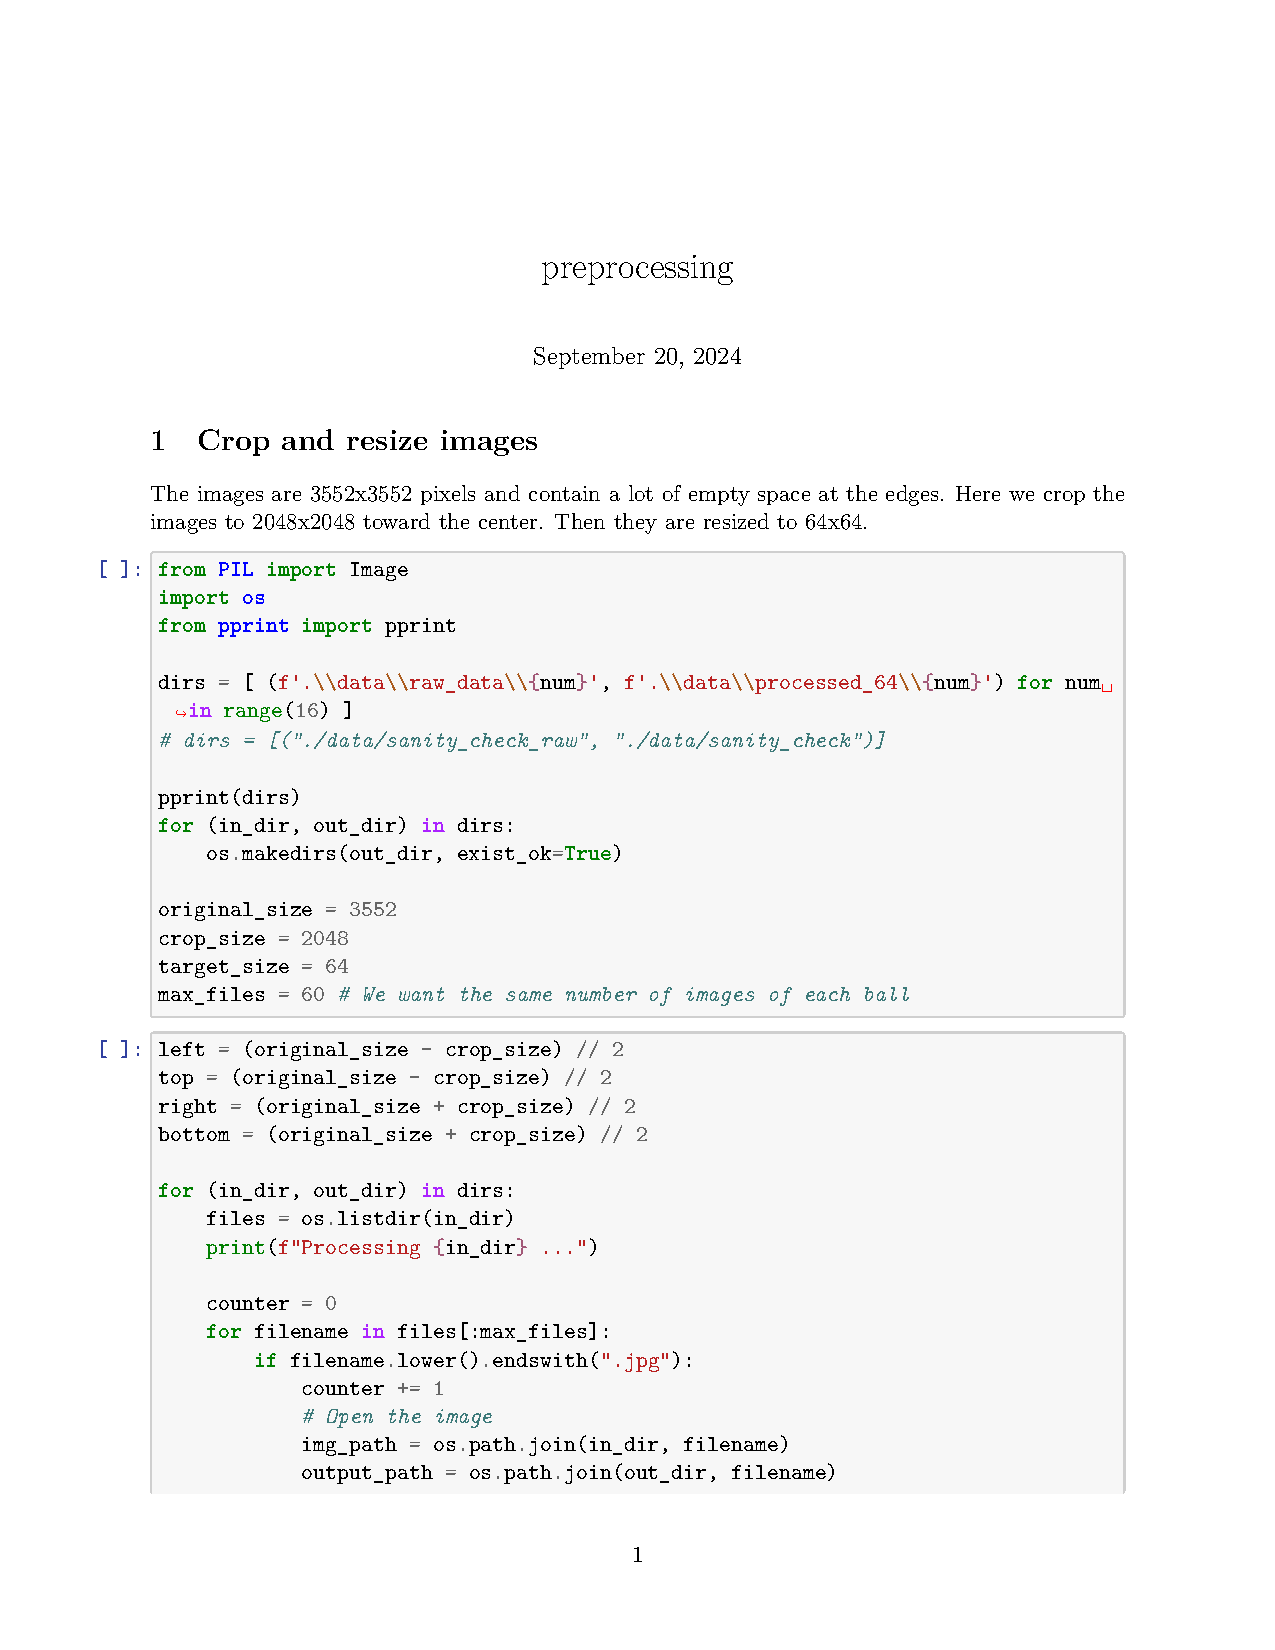
\includepdf[pages=-]{preprocessing.pdf}

\end{document}